\section{The coherence of light}

\begin{otherlanguage}{russian}
	\epigraph{Нахрена нам зеркала, на дворе 20 век.}{Петров М. И.}
\end{otherlanguage}

\subsection{Bunching and antibunching of photons}

Lets consider Michelson stellar interferometer (fig \ref{fig:stellar}). From distant stars the two light beams is coming to our set-up. Light is an electromagnetic wave, so we can write:
\begin{equation}
	\vec{E} = \vec{E}_{\vec{k}} \left( e^{i \vec{k} \vec{r}_{M_1}}  + e^{i \vec{k} \vec{r}_{M_2}} \right) + \vec{E}_{\vec{k}'} \left( e^{i \vec{k'} \vec{r}_{M_1}} + e^{i \vec{k}' \vec{r}_{M_2}} \right).
\end{equation}
If we decide to compute the intensity, we will get (see Scully)
\begin{equation}
	I = \langle \vec{E} \cdot \vec{E}^* \rangle_t  = 4 I_0 \left( 1 + \underbrace{\cos \left[\frac{\left( \vec{k} + \vec{k}' \right) \vec{r}_0}{2}\right]}_{\text{fast term}} \underbrace{\cos \left[\half  k r_0 \varphi \right]}_{\text{slow term}} \right),
\end{equation}
where $\vec{r}_0 = \vec{r}_{M_1} - \vec{r}_{M_2}$, $I_0=\langle \vec{E}_{\vec{k}} \cdot \vec{E}_{\vec{k}}^* \rangle_t=\langle \vec{E}_{\vec{k'}} \cdot \vec{E}_{\vec{k'}}^* \rangle_t$. To make out light and dark spots we need the following condition
\begin{equation}
	k r_0 \varphi \approx \pi \qquad \to \qquad \varphi = \frac{\pi}{k r_0}.
\end{equation}
It means that to change light spot to the dark one  we need $\Delta r_0 = \frac{\pi}{k \varphi}$. So the bigger distance between mirrors $M_1$ and $M_2$, the better resolution we get (we will be able to detect smaller $\varphi$). But there appear to be a lot of technical troubles.
\begin{figure}
	\centering
	
\includegraphics[width=0.5\linewidth]{fig/L3/Ij8NUO6Gat0}
	\caption{wow such Jesus}
	\label{fig:jesus}
\end{figure}

One can chose another pill and built a set up with two distant photodetectors (fig \ref{fig:new_stellar}). Now we don't have annoying mirrors and measure only currents $i_1$ and $i_2$, which are proportional to the intensities $I_1$ and $I_2$ of incident light beams. By this framework we can significantly increase $r_0$ and this will lead to a higher resolution. People who did very precise measurements, noticed that they no longer measure intensities of indecent light, but only noises of almost single photons.


\begin{figure}
	\centering
	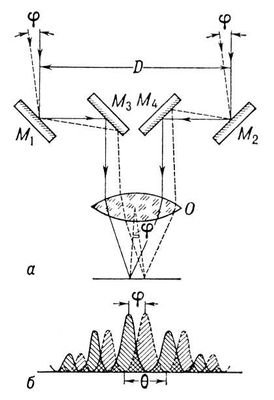
\includegraphics[width=0.6\linewidth]{fig/L3/stellar}
	\caption{A Michelson stellar interferometer}
	\label{fig:stellar}
\end{figure}


\begin{figure}
	\centering
	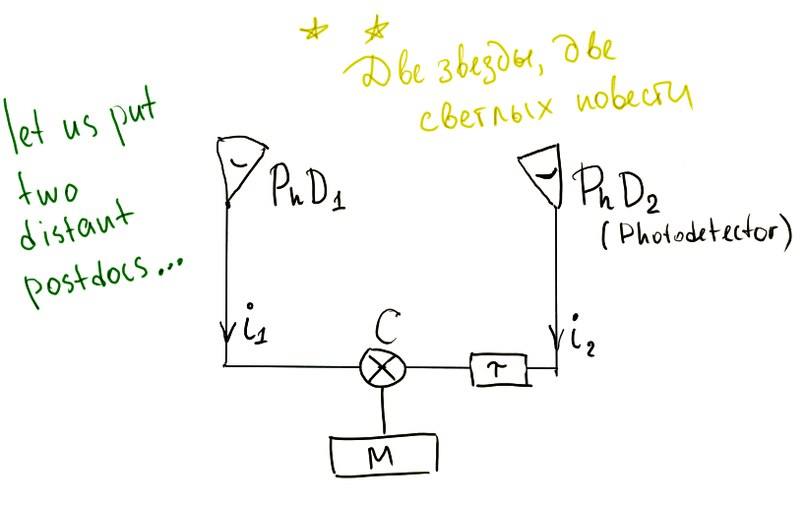
\includegraphics[width=0.8\linewidth]{fig/L3/new_stellar}
	\caption{A symmetric interferometer with distant photodetectors}
	\label{fig:new_stellar}
\end{figure}




Now lets take a look at this situation from a theoretical point of view. Let us compute the following correlator
\begin{equation}
	g^{(2)} = \frac{\langle i_1, i_2 \rangle }{\langle i_1 \rangle \langle i_2 \rangle},
\end{equation}
where
\begin{equation}
	i_1 = \langle i_1 \rangle + \Delta i_1, \qquad i_2 = \langle i_2 \rangle + \Delta i_2, \qquad \langle i_1 \rangle = \langle i_2 \rangle = i_0.
\end{equation}
Then we can write
\begin{equation}
	g^{(2)} = \frac{i_0^2 + \langle \Delta i_1, \Delta i_2 \rangle}{i_0^2} = 1 + \frac{\langle \Delta i_1, \Delta i_2 \rangle}{i_0^2}.
\end{equation}
So in fact one measured the average of $\Delta i_1$ and $\Delta i_2$. To study the issue in more details the so called \textit{HBT experiment} was done. The principle scheme of the set up it shown on fig \ref{fig:HBT_exp}. The heart of the matter is that method allows to avoid the atmospherically sensitive terms (fast terms) like $\cos \left[ \frac{(\vec{k} + \vec{k}') \cdot \vec{r}_0}{2} \right]$.

\begin{figure}
	\centering
	\begin{minipage}[h]{0.70\linewidth}
		\center{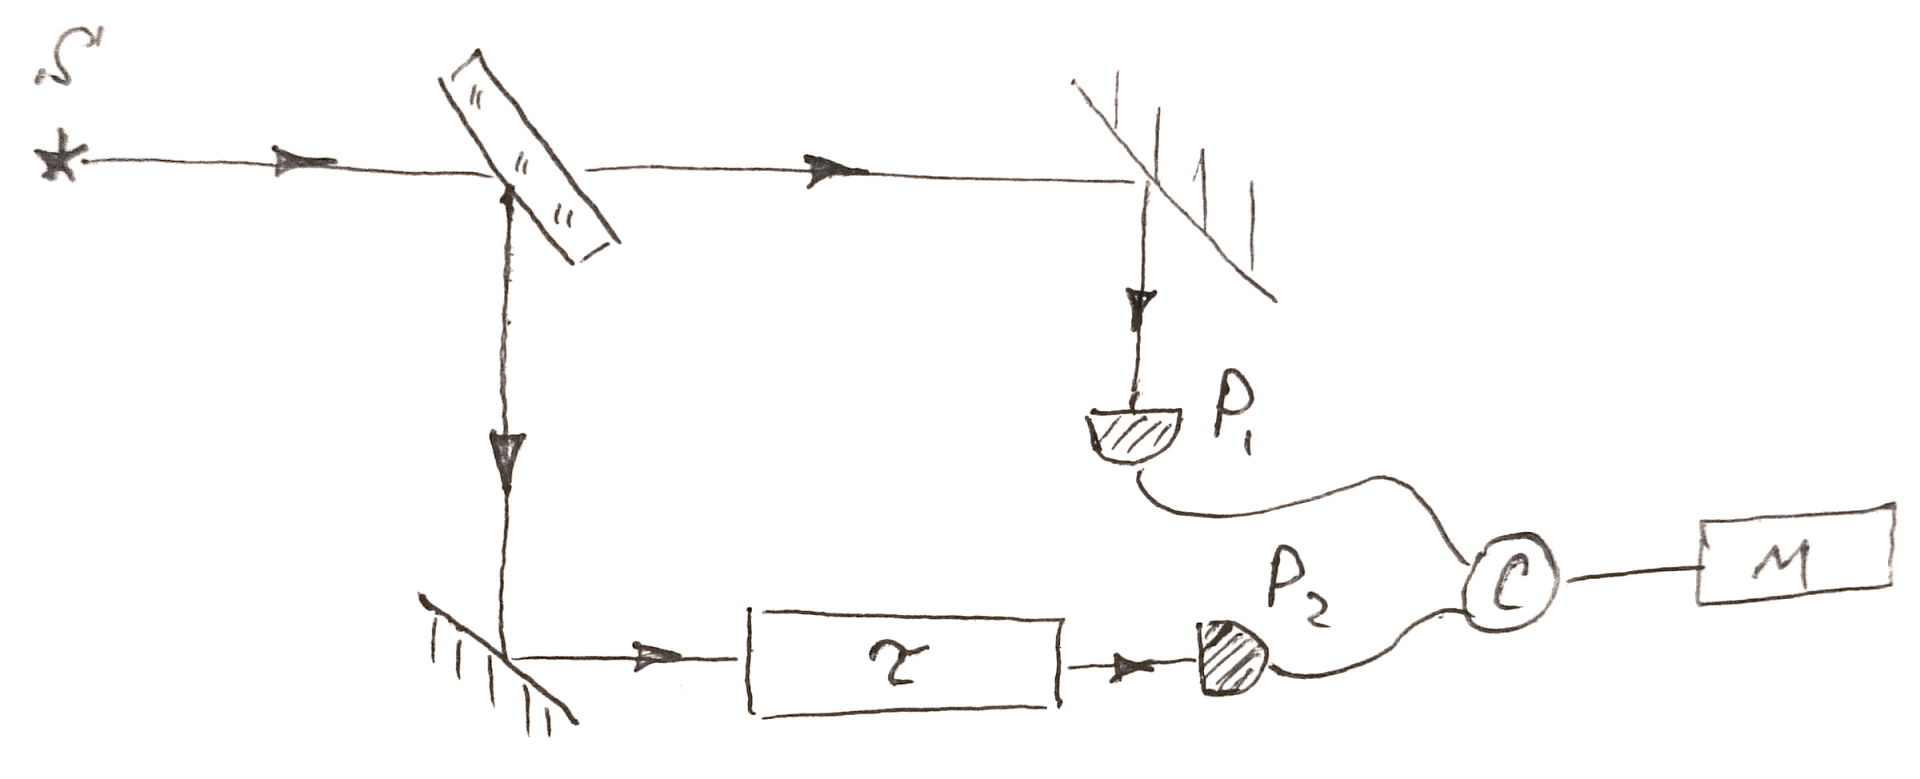
\includegraphics[width=1\linewidth]{fig/L3/HBT_first}} a) Light beam mode\\
	\end{minipage}
	\vfill
	\begin{minipage}[h]{0.7\linewidth}
		\center{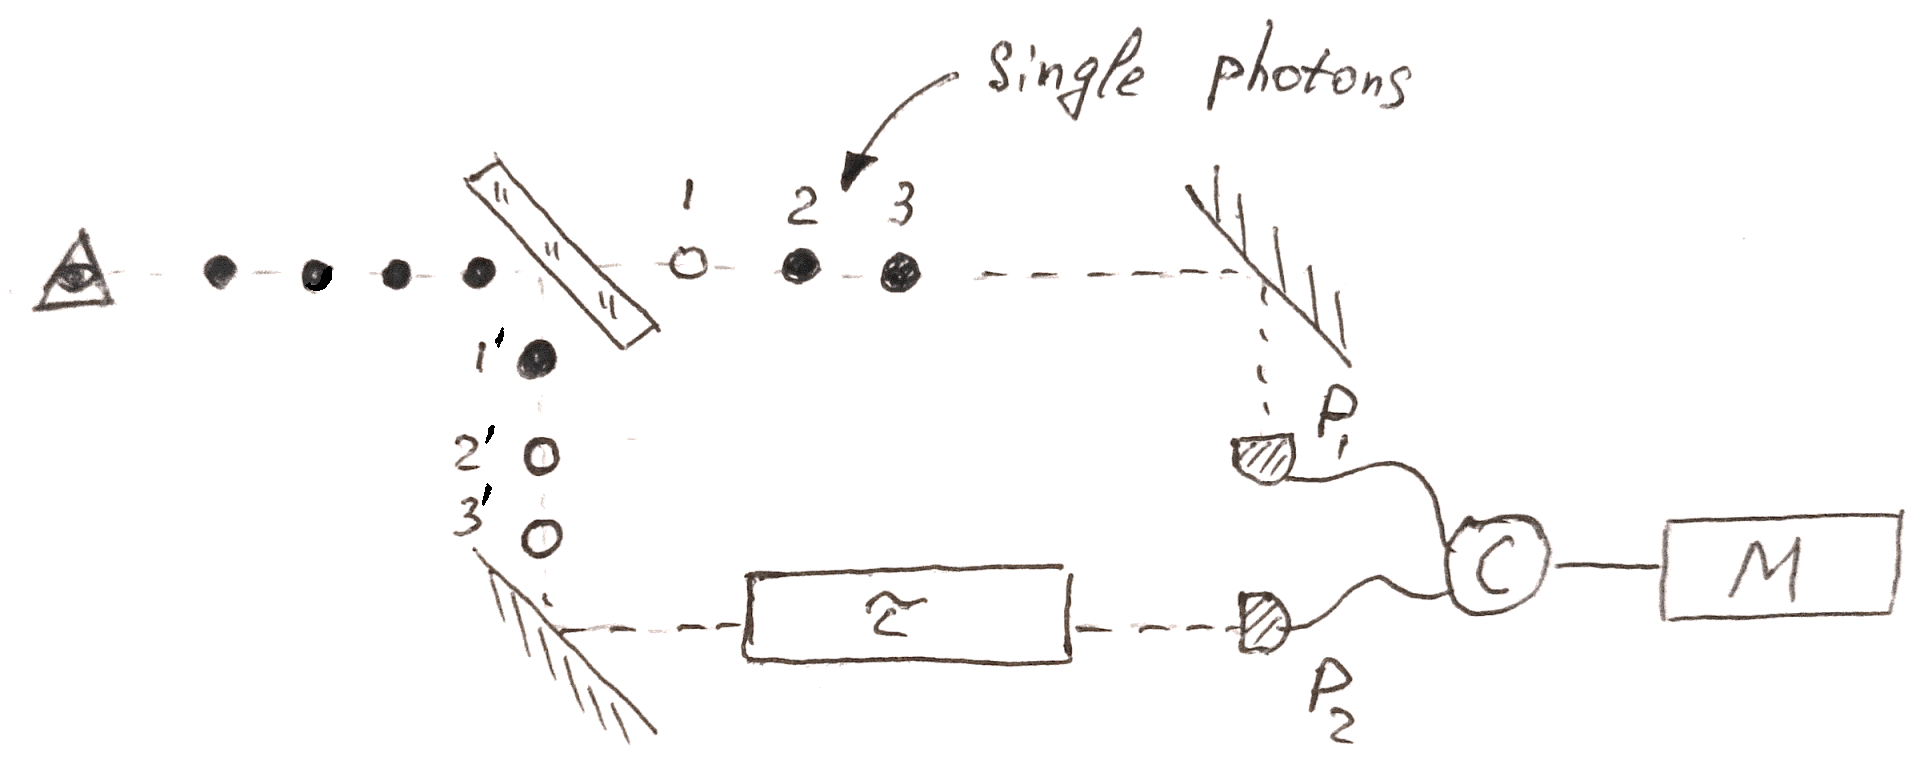
\includegraphics[width=1\linewidth]{fig/L3/HBT_second}} \\b) Single photon mode
	\end{minipage}
	\caption{Schematic diagram of the Hanbury Brown-Twiss intensity interferometer. Here $P_1$ and $P_2$ are photodetectors, $\tau$ is the delay time, $C$ is a multiplier, and $M$ is the integrator}
	\label{fig:HBT_exp}
\end{figure}

Lets analyze the second order correlator:
\begin{equation}
	g^{(2)} (\tau) = 1 + \frac{\langle \Delta i(t) \Delta i (t + \tau) \rangle}{i_0^2}.
\end{equation}
Here can single out some properties:
\begin{enumerate}
	\item $g^{(2)}(0) = 1 + \frac{\langle \Delta i^2 (t) \rangle}{i_0^2} \geq 1 $.
	\item $\lim\limits_{\tau \to \infty} g^{(2)}(\tau) = 1$.
	\item $g^{(2)}(0) \geq g^{(2)}(\tau)$. 
\end{enumerate}
To summarize we could guess that approximate plot of $g^{(2)}(\tau)$ is as it shown of fig. \ref{fig:g2tau_apprx} with a solid line.
\begin{figure}[h!]
	\centering
	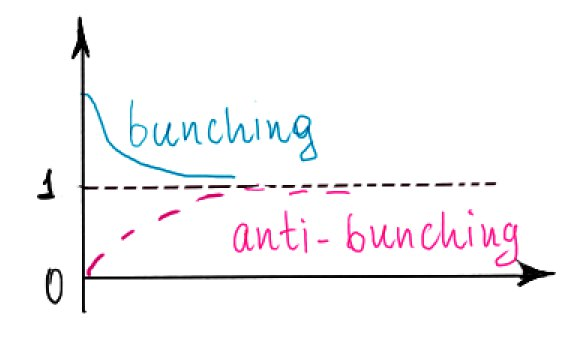
\includegraphics[width=0.5\linewidth]{fig/L3/g2tau_apprx}
	\caption{Approximate plot of $g^{(2)}(\tau)$}
	\label{fig:g2tau_apprx}
\end{figure}

During measuring noises, which were mentioned thereinbefore, experimentalists got the next weird result:
\begin{equation}
	g^{(2)}(\tau) < 1.
\end{equation}
This effect is called \textit{photon bunching}. But a few lines above it was shown that $g^{(2)}(\tau) \geq 1$. How could it be possible? 

Let us consider the same experiments but with a single photons emitter (fig. \ref{fig:HBT_exp} b). Assume $\tau = 0$, so then we calculate how photon at place $1$ is correlated with a photon at place $1'$. If our light source emits discreate photos then single photon cannot be at two places at the same time, so $g^{(2)}(0) = 0$.

\subsection{Quantum theory of photodetection}

Photons are described by field operators
\begin{equation}
	\hat{\vec{E}} = \hat{\vec{E}}^+ + \hat{\vec{E}}^-,
\end{equation}
where
\begin{eqnarray}
	\hat{\vec{E}}^+ = \sum_{\vec{k}} \varepsilon_{\vec{k}} \hat{a}_{\vec{k}} e^{i \vec{k} \vec{r} - i \omega t} \vec{e}_{\vec{k}}, \\
	\hat{\vec{E}}^- = \sum_{\vec{k}} \varepsilon_{\vec{k}} \hat{a}^{\dagger}_{\vec{k}} e^{-i \vec{k} \vec{r} + i \omega t} \vec{e}^*_{\vec{k}}.
\end{eqnarray}

\begin{figure}[h!]
	\begin{minipage}[h]{0.49\linewidth}
		\center{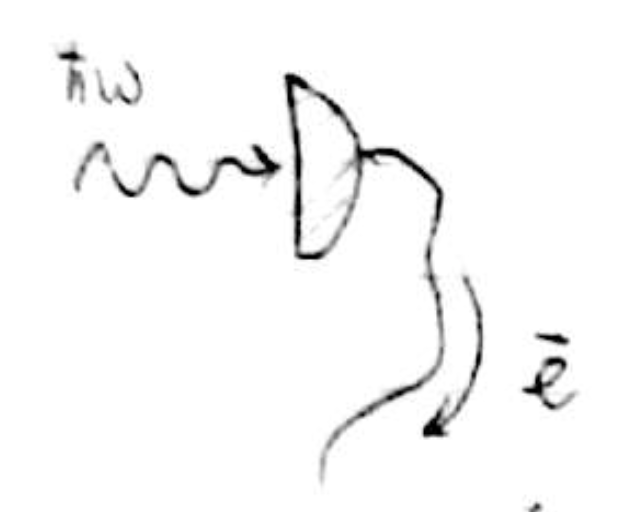
\includegraphics[width=0.6\linewidth]{fig/L3/dec} \\ a)}
	\end{minipage}
	\hfill
	\begin{minipage}[h]{0.49\linewidth}
		\center{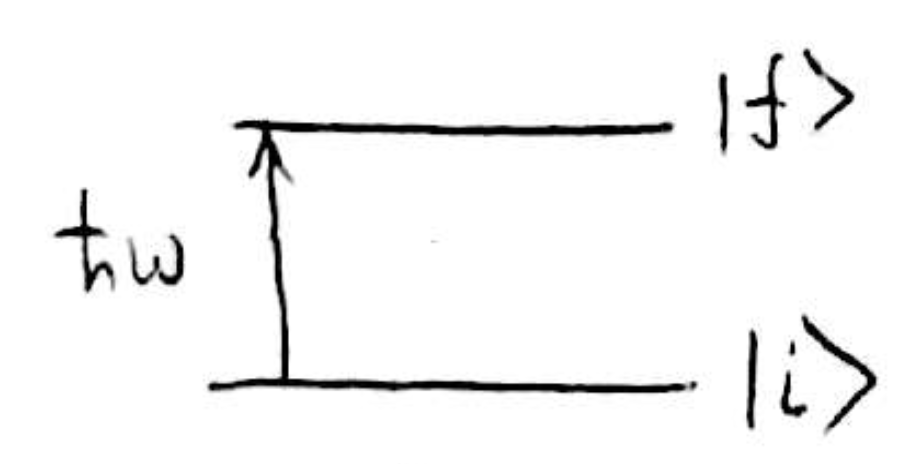
\includegraphics[width=0.7\linewidth]{fig/L3/lev} \\ b)}
	\end{minipage}
	\caption{a) An indecent photon generate an electron which brings current; b) Atom states}
	\label{fig:dec}
\end{figure}


To simplify all the calculations let us consider only \textit{one mode} and only \textit{one linear polarisation} of field:
\begin{equation}
	\hat{\vec{E}}^+ = \hat{E}^+ \vec{e}_{\vec{k}}.
\end{equation}
When an indecent photon got absorbed, it excites the atom detector: $\ket{i} \to \ket{f}$ (see fig. \ref{fig:dec}, b).


The probability of  absorption of one photon (= the probability of detection of one photon) depends only on operator $\hat{E}^+$ due to detection principle (see fig. \ref{fig:dec}). The transition probability of the detector atom for absorbing a photon from the field at position $\vec{r}$ between times $t$ and $t+dt$ is proportional to $\omega_1(\vec{r},t) dt$, with
\begin{equation}
	\omega_1 (\vec{r}, t) = \sum_{f} \left| \bra{f} \hat{E}^{+} \ket{i} \right|^2 = \sum_{f} \bra{i} \hat{E}^{-} \ket{f} \bra{f} \hat{E}^{+} \ket{i} = \bra{i} \hat{E}^-(\vec{r},t) \hat{E}^+ (\vec{r},t) \ket{i}.
\end{equation}
Here the $\sum_{f} \ket{f} \bra{f} = 1$ relation was used.

Shall us define the first-order correlation function
\begin{equation}
	g^{(1)} (\vec{r}_1,t_1; \vec{r}_2, t_2) \sim \bra{i} \hat{E}^-(\vec{r}_1, t_1) \hat{E}^+ (\vec{r}_2, t_2) \ket{i} = \langle \hat{E}^-(\vec{r}_1, t_1) \hat{E}^+ (\vec{r}_2, t_2) \rangle.
\end{equation}
It is useful for quantifying the coherence between two electric fields, as measured in a Michelson or other linear optical interferometer. Here we used the average notation as 
\begin{equation}
	\langle \hat{A} \rangle \myeq \bra{i} \hat{A} \ket{i}.
\end{equation}

The detection probability of two photons is given by
\begin{multline}
	\omega_2 (\vec{r}_1, t_1; \vec{r}_2, t_2) = \sum_{f} \left| \bra{f} \hat{E}^+ (\vec{r}_1 ,t_1) \hat{E}^+ (\vec{r}_2 , t_2) \ket{i} \right|^2 = \\ = \bra{i} \hat{E}^- (\vec{r}_2 , t_2) \hat{E}^- (\vec{r}_1 , t_1) \hat{E}^+ (\vec{r}_1 , t_1) \hat{E}^+ (\vec{r}_2 , t_2) \ket{i}.
\end{multline}
The joint probability of photodetection is thus governed by the second-order correlation function:
\begin{equation}
	g^{(2)}(\vec{r}_1, t_1; \vec{r}_2, t_2) = \frac{\langle \hat{E}^-(\vec{r}_2, t_2) \hat{E}^-(\vec{r}_1, t_1) \hat{E}^+(\vec{r}_1, t_1) \hat{E}^+(\vec{r}_2, t_2)\rangle}{\langle \hat{E}^-(\vec{r}_2, t_2) \hat{E}^+(\vec{r}_2, t_2) \rangle \langle \hat{E}^-(\vec{r}_1, t_1) \hat{E}^+(\vec{r}_1, t_1) \rangle}.
\end{equation}
It refers to intensity (e.g. for currents). The exact expression for the first-order correlation function is the following:
\begin{equation}
	g^{(1)} (\vec{r}_1, t_1; \vec{r}_2, t_2) = \frac{\langle \hat{E}^-(\vec{r}_1, t_1) \hat{E}^+ (\vec{r}_2, t_2) \rangle}{\sqrt{\langle \hat{E}^-(\vec{r}_2, t_2) \hat{E}^+(\vec{r}_2, t_2) \rangle \langle \hat{E}^-(\vec{r}_1, t_1) \hat{E}^+(\vec{r}_1, t_1) \rangle}}.
\end{equation}
In fact it refers to interference in quantum mechanic.

A particular case is often used, precisely a case $\vec{r}_1 = \vec{r}_2$ and $\tau = t_2 - t_1$. In such case notation is $g^{(2)} (\vec{r}_1, t_1; \vec{r}_2, t_2) \myeq g^{(2)} (\tau)$. So we have
\begin{equation}
	g^{(2)} (\tau) = \frac{\langle \hat{E}^-(\tau) \hat{E}^-(0) \hat{E}^+(0) \hat{E}^+(\tau)\rangle}{\langle \hat{E}^-(0) \hat{E}^+(0) \rangle^2},
\end{equation}
where $\langle \hat{E}^-(0) \hat{E}^+(0) \rangle = \langle \hat{E}^-(\tau) \hat{E}^+(\tau) \rangle$, $\forall \tau$ was used which means that the signal is homogeneous. For a case of only \textit{one mode field} we can write
\begin{equation}
	g^{(2)} (\tau) = \frac{\langle \hat{a}^{\dagger} (\tau) \hat{a}^{\dagger} (0) \hat{a}(0) \hat{a}(\tau) \rangle}{\langle \hat{a}^{\dagger} \hat{a} \rangle^2}.
\end{equation}
Important to notice that in numerator of fraction is \textit{normally ordered}.

\begin{testexample}[The second-order correlation function for Fock states ($\ket{i} = \ket{n}$).]
	%\textcolor{red}{(UNCOMMENT THIS LATER! (see source))}
	\begin{equation}
		g^{(2)} (0) = \frac{\bra{n} \hat{a}^{\dagger} \hat{a}^{\dagger} \hat{a} \hat{a} \ket{n}}{\bra{n}\hat{a}^{\dagger} \hat{a} \ket{n}} = \frac{n(n-1)}{n^2} = 1 - \frac{1}{n} < 1, \quad \forall n.
	\end{equation}
	This is a factor of a single-photon beam, e.g. $n=1 \to g^{(2)}(0)=0$. Exactly this effect was observed in a HBT experiment!
\end{testexample}

\begin{hw}[The second-order correlation function for coherent states.]
	Compute $g^{(2)}(0)$ for case $\ket{i} = \ket{\alpha}$.
\end{hw}